\section{Background}
\label{sec:background}

\subsection{Task-Oriented Dialog System}
The architecture of a task-oriented dialog system
for shopping guide assistant is illustrated in \figref{fig:dialog_system}.
It consists of three components like common dialog system, natural
language understanding (NLU), dialog management
(DM), and natural language generation (NLG).
In addition, the system also interacts with a product search engine
for the purpose of shopping guide. 
\begin{figure}[h]
	\centering
	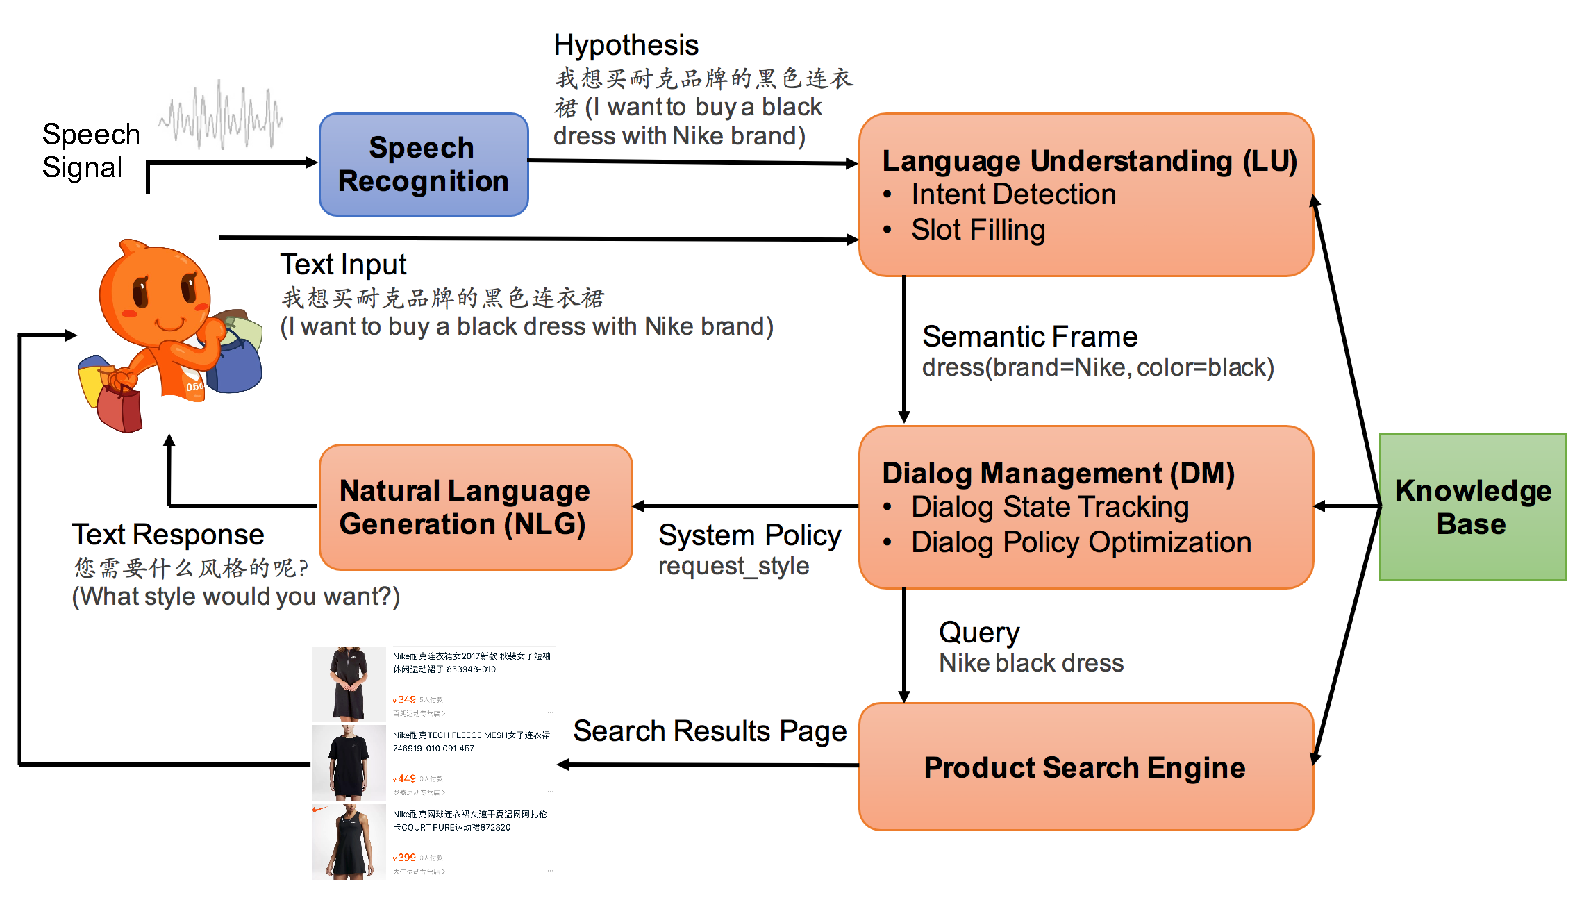
\epsfig{file=figures/dialog_system.eps, width=1\columnwidth}
	\caption{Pipeline framework of task-oriented dialog system for shopping guide assistant.}
	\label{fig:dialog_system}
	\vspace{-10pt}
\end{figure}

NLU contains modules of Intent Detection and Slot Filling.
Intent Detection aims to predict which product category user is going to buy,
such as dress or t-shirt and so on.
Our work in this paper focus on optimizing Slot Filling
and we will detailed introduce in the following sections.

\subsection{Slot Filling}
\label{sec:slot_filling}
A major task in natural language understanding (NLU) is to extract semantic constituents
by searching input text to fill in values for predefined slots in a semantic frame \cite{mesnil2015using},
which is often referred to as slot filling.
The slot filling task can also be viewed as assigning
an appropriate semantic label to each word in
the given input text.

In the below example (in \tabref{tab:slot_filling_demo}) from our corpus following the popular in/out/begin (IOB) annotation method,
``\emph{耐克 (Nike)}'' is labeled as brand property (\textbf{B-Brand}/\textbf{I-Brand}) and ``\emph{黑色 (black)}'' is labeled as color property (\textbf{B-Color}/\textbf{I-Color})
according to the slot labels from Knowledge-Base.
They are all classified as Property Value type.
``\emph{连衣裙 (dress)}'' and ``\emph{品牌 (brand)}'' are Category type (\textbf{B-CATEGORY}/\textbf{I-CATEGORY})
and Property Key type (\textbf{B-PK}/\textbf{I-PK}) respectively which are Name Entity types.
Thus, there are three Name Entity types including \emph{Category}, \emph{Property Key} and \emph{Property Value}.
Other words in the example utterance that carry no semantic meaning are assigned \textbf{O} label.

The semantic labels are defined by an extern Knowledge-Base. 
For example in the dress category, there are 26 semantic labels,
they totally describe the different properties for a dress,
so that we classify them as Property Value (\textbf{PV}) type.
Addition to Property Key (\textbf{PK}) type, Category (\textbf{CATEGORY}) type and \textbf{O} label,
there are totally 29 (57 for IOB format) slot labels (refer to \tabref{tab:slot_labels}).
Compared to the most well-known dialog state tracking challenge (DSTC) dataset,
in which there are only 9 slot labels in DSTC1\footnote{\url{http://research.microsoft.com/en-us/events/dstc/}} for bus booking scene
and 8 slot labels in DSTC2\footnote{\url{http://camdial.org/~mh521/dstc/}} for restaurant booking scene.
Our dataset has much larger amount of slot labels (totally 29),
so that we call it a large scaled slot filling problem.

\begin{table*}[htbp]
	\label{tab:slot_filling_demo}
	\caption{Sample from our corpus with slot annotation (IOB format).}
	\centering
	\scriptsize
	\begin{tabular}{c|c|c|c|c|c|c|c|c|c|c|c|c|c}
		\toprule
		\multirow{2}{*}{Utterance} & 我 & 想 & 买 & 耐 & 克 & 品 & 牌 & 的 & 黑 & 色 & 连 & 衣 & 裙 \\
		\cmidrule{2-14}
		& \em{I} & \em{want} & \em{buy} & \multicolumn{2}{c|}{\em{Nike}} & \multicolumn{2}{c|}{\em{brand}} & $\backslash$  & \multicolumn{2}{c|}{\em{black}} & \multicolumn{3}{c}{\em{dress}} \\
		\midrule
		Slots & \textbf{O} & \textbf{O} & \textbf{O} & \textbf{B-Brand} & \textbf{I-Brand} & \textbf{B-PK} & \textbf{I-PK} & \textbf{O} & \textbf{B-Color} & \textbf{I-Color} & \textbf{B-CATEGORY} & \textbf{I-CATEGORY} & \textbf{I-CATEGORY} \\
		\bottomrule
	\end{tabular}
	\vspace{-10pt}
\end{table*}

\begin{table}[htbp]
	\label{tab:slot_labels}
	\caption{}
	\centering
	\scriptsize
	\begin{tabular}{c|c|c|c}
		\toprule
		Name Entity & PV & PK & CATEGORY \\
		\midrule
		Slot Label & \textbf{Color}, \textbf{Brand}, ... & \textbf{PK} & \textbf{CATEGORY} \\
		\midrule
		Example Term & \emph{black}, \emph{Nike}, ... & \emph{brand}, \emph{color}, ... & \emph{dress}, \emph{t-shirt}, ... \\
		\bottomrule
	\end{tabular}
	\vspace{-10pt}
\end{table}

Given an utterance consisting of a sequence of
words $\textbf{w} = (w_1, w_2, ..., w_T)$,
the goal of slot filling
is to find a sequence of slot labels $\textbf{s} = (s_1, s_2, ..., s_T)$, one for each word in the utterance, such that:
\begin{equation}
	\hat{\textbf{s}} = \mathop{\arg\max}_{\textbf{s}}P(\textbf{s}|\textbf{w}).
\end{equation}

\subsection{RNN Sequence Labeling}
Slot filling is typically treated as a sequence labeling
problem. Sequence models including conditional
random fields \cite{raymond2007generative} and RNN models \cite{yao2014spoken,mesnil2015using} are among
the most popular methods for sequence labeling
tasks. \figref{fig:model}(a) shows the principle architecture of a BiLSTM-CRF model which is
the state-of-the-art model for various sequence labeling tasks \cite{huang2015bidirectional,reimers2017optimal}.
BiLSTM-CRF model includes BiLSTM layer and CRF layer. 

%\begin{figure}[h]
%	\centering
%	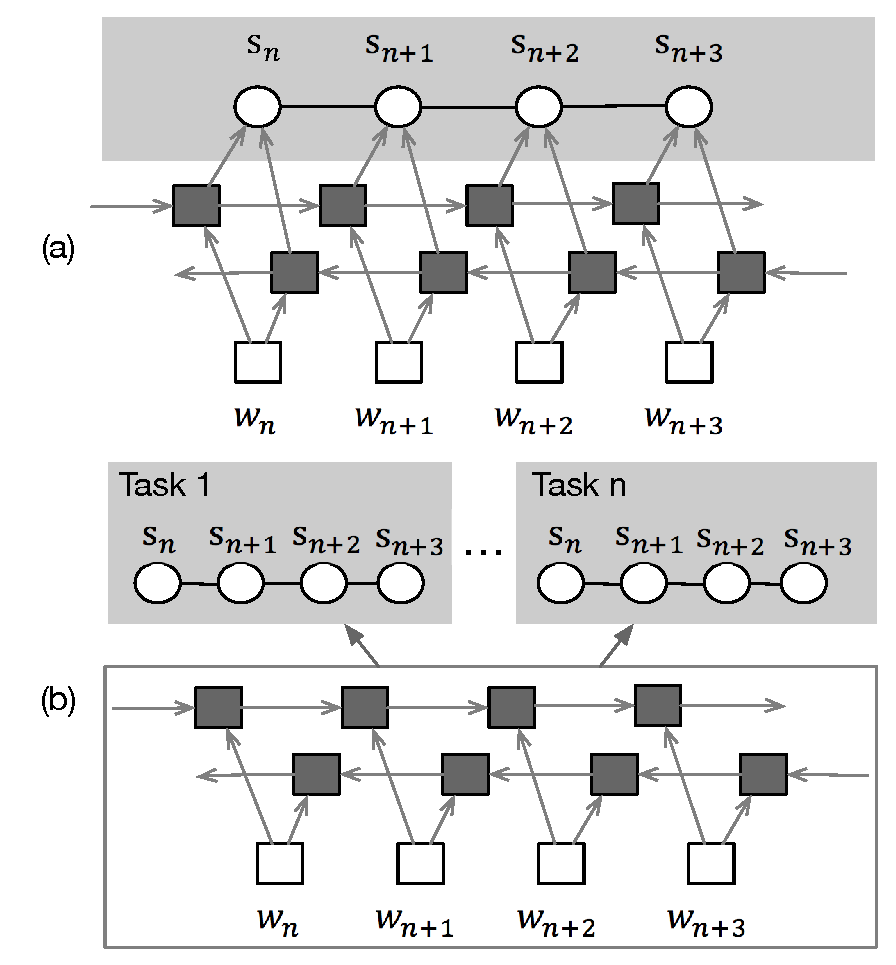
\epsfig{file=figures/bilstm_crf_related.eps, width=0.8\columnwidth}
%	\caption{(a) Basic BiLSTM-CRF model. (b) Multi-task learning with BiLSTM-CRF model, in which different tasks share the parameters.}
%	\label{fig:bilstm_crf_related}
%	\vspace{-10pt}
%\end{figure}

Bidirectional LSTMs enable the
hidden states to capture both historical and future
context information of the words. 
Mathematically, the input of this BiLSTM layer
is a sequence of word representations
(vectors) for the input utterance $\textbf{w}$,
denoted as $(\bi{x}_1, \bi{x}_2, ..., \bi{x}_T)$.
The output of this BiLSTM layer is a sequence of the hidden
states for each input word, denoted
as $(\bi{h}_1, \bi{h}_2, ..., \bi{h}_T)$.
Each final hidden state is the concatenation of the forward
$\overrightarrow{\bi{h}_i}$ and backward $\overleftarrow{\bi{h}_i}$ hidden states. We know that
\begin{eqnarray*}
	& \overrightarrow{\bi{h}_i} = LSTM(\bi{x}_i, \overrightarrow{\bi{h}_{i-1}}),
	 \overleftarrow{\bi{h}_i} = LSTM(\bi{x}_i, \overleftarrow{\bi{h}_{i+1}}), \\
	& \bi{h}_i = [\overrightarrow{\bi{h}_i};\overleftarrow{\bi{h}_i}].
\end{eqnarray*}
Most of time we use a Stacking BiLSTM fashion to make the model deeper,
%in which higher layer takes the output state $\bi{h}_i$ of the connected lower layer as input.
in which the output $\bi{h}_i^l$ of layer $l$ becomes the input of layer $l+1$.

It is almost always beneficial to consider the correlations
between the current label and neighboring
labels since there are many syntactical constrains
in natural language sentences. For example,
\textbf{I-Brand} will never follow a \textbf{B-Color}. If
we simply feed the above mentioned hidden states
independently to a Softmax layer to predict the labels\cite{hakanni-tur2016multidomain},
then such constrains will not be more likely
to be broken. Linear-chain Conditional Random
Field is the most popular way to control the structure
prediction and its basic idea is to use a series
of potential function to approximate the conditional
probability of the output label sequence
given the input word sequence.

Formally, we take the above sequence of hidden
states $\bi{h} = (\bi{h}_1, \bi{h}_2, ..., \bi{h}_T)$
as our input to the CRF layer,
and its output is our final prediction label sequence
$\bi{y} = (y_1, y_2, ..., y_T)$,
where $\bi{y}$ is in the set of all possible labels $\bi{s}$.
We denote $\mathcal{Y}(\bi{h})$ as the set of all possible label sequences.
Then we derive the conditional probability of the output sequence
given the input hidden state sequence is
$$
p(\bi{y}|\bi{h};\bi{W})= ... ,
$$
where $\bi{W}$ is the weight matrices,
and the subscription indicates that we extract the
weight vector for the given label pair $(y_{i-1}, y_i)$.
To train the CRF layer, we use the classic maximum
conditional likelihood estimation to train our
model. The final log-likelihood with respect to the
weight matrices is
$$
L(\bi{W}) = .
$$
Finally, we adopt the Viterbi algorithm for decoding the optimal output sequence $\bi{y}^{*}$.